% !TeX spellcheck = en_US
\documentclass[11pt,a4paper]{article}
\usepackage[utf8]{inputenc}
\usepackage{amsmath}
\usepackage{amsfonts}
\usepackage{amssymb}
\usepackage{graphicx}
\usepackage{mathtools}
\usepackage[hidelinks]{hyperref}  % most people dont know of this :3

\usepackage[backend=bibtex,style=verbose-ibid]{biblatex}
\addbibresource{citations.bib}

\usepackage{listings}
\usepackage{color}
\definecolor{dkgreen}{rgb}{0,0.6,0}
\definecolor{gray}{rgb}{0.5,0.5,0.5}
\definecolor{mauve}{rgb}{0.58,0,0.82}

\lstset{frame=tb,
  language=Python,
  aboveskip=3mm,
  belowskip=3mm,
  showstringspaces=false,
  columns=flexible,
  basicstyle={\small\ttfamily},
  numbers=none,
  numberstyle=\tiny\color{gray},
  keywordstyle=\color{blue},
  commentstyle=\color{dkgreen},
  stringstyle=\color{mauve},
  breaklines=true,
  breakatwhitespace=true,
  tabsize=3
}


\newcommand{\inv}{^{\raisebox{.2em}{$\scriptscriptstyle-1$}}}
\newcommand{\qed}{\hfill $\blacksquare$}

\newcommand{\integers}{\mathbb{Z}}
\newcommand{\rationals}{\mathbb{Q}}
\newcommand{\reals}{\mathbb{R}}
\newcommand{\complexes}{\mathbb{C}}
\newcommand{\field}{\mathbb{F}}

\author{Jacob Bruner}
\title{IB Extended Essay}
\date{\today}

\begin{document}
\maketitle
\tableofcontents

\pagebreak

\iffalse
############
heres an example of a code block
\begin{lstlisting}
        def intervalValues(z, n):
            return output # return the sequence of values
\end{lstlisting}

heres an example of an image
\begin{figure}[h]
\begin{center}
\includegraphics[scale=.37]{onefifteen} 
\caption{Sequences Generated by n = 1-15 on Argand Diagram}
\end{center}
\end{figure}
############
\fi

\section*{Foreword}

This paper is for expository purposes only. Although the information presented is accurate, you should never implement a cryptographic system yourself unless you know \textit{\emph{exactly}} what you're doing. \textbf{I am not liable for any damages caused in testing/creating/implementing any cryptographic protocol referenced in this paper.} Cryptography's greatest weakness is human-error, and virtually \textit{all} cryptographic breaks result from poor implementation. 

\section{Introduction and Aim}
\subsection{Motivating Problem}
It's undeniable that our modern-day world is reliant on cryptography. Every time a phone sends a text, a browser connects to a server, an email gets sent off, a monetary transaction is made, and much much more, our devices are, unbeknownst to us, performing many hundreds of math operations to ensure our data are 'encrypted.' 
% ? In fact, your device is likely doing it right now. 
But what does 'encryption' mean? Let's introduce some definitions. ‘Encryption’ is the process of disguising a message to be, loosely speaking, hidden to all but the intended recipient. This is the process of converting a ‘plaintext’ message into a jumbled ‘ciphertext’, which can be readily shared without risk of the sensitive message leaking. Converting a plaintext message (typically a string/list of characters) into a ciphertext is known as an ‘enciphering’ or ‘encrypting’ transformation. Likewise the reverse operation of recovering the plaintext message from a ciphertext is known as the \textit{deciphering transformation.}\autocite[54]{koblitz} If we denote the plain and cyphertext $\mathcal{P}$ and $\mathcal{C}$ respectively and the enciphering map $f$ and its inverse $f\inv$ we obtain the following diagram:

$$ \mathcal{P} \overset{f}\longrightarrow \mathcal{C} \overset{f\inv}\longrightarrow \mathcal{P} $$

The intuitive way to implement this cryptosystem has the two transacting parties agree upon the nature of the map $f$ in secret, beforehand. This might mean meeting up with a friend in-person to establish the common secret, $f$ and $f\inv$, so that you could encrypt and decrypt each other's emails—fending off any prying eyes accessing their emails. This type of system has a special name, \textit{"Symmetric Key Cryptography"}, reflecting the fact that both parties have the same shared secret (foreshadowing). Important historical examples include the 'Caeser Cipher' (supposedly invented by \textit{the} Julius Caeser)%citation?
, where $f$ is a shift operation that maps each letter to a new one a number of places ahead or behind. For instance, the two parties might decide beforehand the map $f$: \textit{shift each character forward in the alphabet 3 letters}, implying the inverse map $f\inv$: \textit{shift each character back 3 letters}. This might look like so: \footnote{The informed reader will notice that Ceaser Ciphers are really just linear transformations in disguise, provoking thought into whether more advanced techniques could be used. For instance, we could consider groups of two letters, called \textit{digraphs}, resulting in $f$ being a 2x2 invertible matrix, encoding the shift in a two-by-two matrix. Similarly, we could consider invertible \textit{affine} transformations of the form $f:x \to Ax + \vec{b}$, where A encodes a certain scaling factor.}

\begin{align*}
 \mathcal{P} &\sim A,B,C,D,E,F,…Y,Z  \\ 
 \mathcal{C} &\sim D,E,F,G,H,I,…B,C 
\end{align*} % I'm not sure what symbol to use here...Equivalance relation? Monomorphism?
And, for example, if you wanted to encrypt the message $\mathcal{P} =$ "HELLO", you would obtain the ciphertext $\mathcal{C} =$ "KHOOR" which you would promptly send off for your friend to decode with the inverse, subtract-three-letters map. Note that, even in this simple example, repeated letters, word length, and other syntactic information provide a lot of information about the nature of the plaintext. Although this is a trivial example, schemes which, loosely speaking, encode any information about the syntax (or related notions) of the plaintext are usually highly vulnerable to a technique called \textit{differential cryptanalysis},which, at a high level, measures the change in cyphertext given a change in input, primarily targeting published symmetric-key protocols.\autocite[56]{koblitz} 

To see what a caeser cipher looks like mathematically, we start encoding each letter as a number from 0, which is A, to 25, which is Z. Of course this depends on what alphabet one uses, if one chooses to include spaces, numbers, punctuation etc. We can represent the operation that takes a letter and maps it $n$ places ahead with addition. Importantly, this operation must 'wrap around' back to zero if you try to exceed 'z' in the alphabet. This process, known as \textit{'modular arithmetic'}, is like circling a clock, where after reaching twelve, the hour hand wrap back around to 1, but we start from 0 instead of 1. So, in our case, shifting 'z' by 3 letters looks like so: $25 + 1 \bmod 26 \equiv 0$, which reads "25 plus 1 \textit{is congruent to} 0 \textit{modulo} (or \textit{mod}) 26." With this in mind, we obtain for each letter $p \in \mathcal{P}$:  

\[
f(p) = p + n \bmod 26 
\]



% I could maybe talk about affine cryptosystems here if I need more words.
% I could also show the linear algebra point of view

Representing a shifting of each letter in the plaintext by $n$ places in the alphabet. Now clearly this isn't a very sophisticated cryptographic scheme... For instance, performing a frequency analysis and comparing the most commonly occurring letters to those of the English alphabet, easily breaking these types of cyphers, broadly referred to as 'substitution ciphers.'\autocite[54]{koblitz} Modern schemes typically employ more resistant techniques, namely where changing just one letter of plaintext often yields a completely different ciphertext, making modern techniques all but impervious to frequency analysis. (Unless someone \textit{really} screwed up an implementation)
  
  For instance, AES encryption, part of the modern web standard, is an example of a '\textit{block substitution cypher},' which are beyond the scope of this paper. % much to my chagrin :(
At a high level, it combines techniques similar to our Caesar Cipher with certain affine (think scaling and transforming) maps performed on blocks of plaintext. It's certainly more complicated than that, but essentially boils down to our system plus some advanced techniques making it resistant to cryptanalysis. (Like permutations, combinations, text look-up-tables and more.) In general, Symmetric-key cryptography (\textit{viz.} predetermined, shared secret) is well understood. For instance, Claude Shannon (\textit{the} definitive father of information theory) proved mathematically that the so-called \textit{'one-time-pad'} encryption technique was completely and utterly unbreakable. 
If a random-generated key is at least as long as the plaintext (specifying a unique, random\footnote{There is a paramount distinction between \textit{random} and \textit{psuedorandom}, the latter of which is vastly easier to implement on a computer. True randomness has to be derived from a non-computer source (for the most part). Commonly implemented approximates include taking the least-significant-digit of a mouse position, or the frequency of keypresses, etc. A one-time-pad–like scheme generated from a psuedorandom source \textit{is} breakable, although usually not without some effort.}, performing modular addition (i.e., wrapping around so as to not exceed the alphabet) on each letter by the private key yields a ciphertext that is uncrackable.\autocite{claude} Although modern systems seek smaller key sizes for performance reasons, this worst-case scenario should demonstrate the strength of symmetric-key algorithms in general. The 'one-time-pad' gets its name from its use in WWII when the KGB would distribute palm-sized pads with these one-time-keys and a table to ease in conversion. Such pads were often made of flammable materials to be burned with no trace.\autocite{lewand} 
  
\begin{figure}[h]
\begin{center}
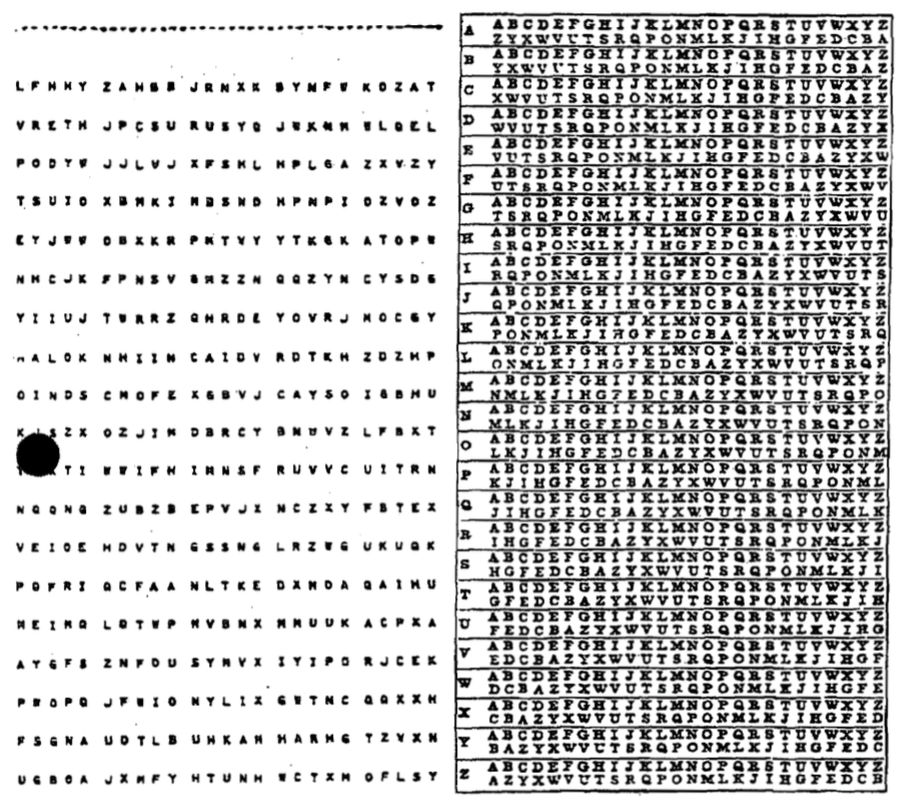
\includegraphics[scale=.29]{images/diana} 
\caption{Format of a one-time-pad used by the NSA\autocite{diana}}
\end{center}
\end{figure}
  

\subsection{The 'Public-Key' Paradox}

In the modern world, it's impractical to require that every shared secret be determined ahead of time. If a user wants to connect to a twitter server over a secure connection, how could symmetric-key encryption be employed? More generally, if two computers want to establish a connection for the first time, is there any way they could do so in an encrypted matter? The intuitive answer might be no, since how could you pass (or otherwise determine) a shared secret without any man-in-the-middle being able to obtain that same key. But this defys the ubiquity of encryption on the internet—every time I connect to a unfamiliar website, I still see a padlock on my browser. How can this be?

Consider the intuitive fact that some operations are more difficult to do in reverse than fowards—certain 'one-way functions.' For instance, if I mixed two different-colored paints together and asked whether you, \textit{a priori}, could deduce the two initial colors given the end result, would you be able to? Although its quite easy to check whether any two colors combine to match the end result, there isn't an easy operation that takes the end result and returns the initial colors. This happens to be true for a number of operations. 

[I have yet to finish this section.]

\section{What is 'Public-Key' Cryptography}
"In applied contexts, the terms "easy" and "hard" are usually interpreted relative to some specific computing entity; typically "cheap enough for the legitimate users" and "prohibitively expensive for any malicious agents"."

The first protocol developed to address this motivating problem was RSA encryption. Leveraging intuitive properties of numbers, RSA establishes our idea of ‘one-way operations’ using simple multiplication of large, highly prime (minimal divisors), numbers. 

\footnote{Although this isn't a true "public-key" algorithm, DH can be easily modified to send arbitrary messages in a scheme known as 'Elgamal encryption.'\\\autocite{elgamal}}

[I have yet to finish this chapter. This will detail Diffie-Hellman key exchange over finite fields, discussing eucliean algorithm/bezouts id to compute inverses. I will then hint towards group theory before transitioning to the introduction.]

\section{How can we formalize this: An Introduction to Groups}
[a word to whoever is reading: I wrote this section before the preceeding sections, so it lacks many critical references to what I have been discussing throughout the paper. In the case of linear or affine cryptosystems, they correspond highly to additive groups $\integers / n \integers$ (n not necessarily prime), and, I believe, direct sums of such (for digraphs, trigraphs, etc). Similarly, Diffie Hellman is secretly group theory in disguise since it concerns itself with fields comprised $(\integers / p \integers, +, \times)$ Upon rereading, I see I jump into fairly complicated math fairly quickly.]

Group theory is the study of symmetry. Every set of symmetries on an object correspond to a group, and likewise every group corresponds to a set of symmetries.\footnote[2]{This is rigorously true if we consider the set of all automorphisms of an object (viz. the set of all bijective maps from and to itself), this forms a group under function composition with the inverses being the inverse maps and the identity being the identity "do nothing" map, so this perspective is justified.} % hmm
Now to unpack what this means, it might be helpful to depict precisely what 'symmetry' is. The prototypical example is geometric symmetry. If we consider the set of symmetries of a square under rotations and reflections, we can form a group with a fancy name, the 'Dihedral group of order 8,' denoted $\mathrm{D}_8$. %More generally, the group of symmetries of an n-gon form the Dihedral group of order 2n, $\mathrm{D}_{2n}$.
(Order, here, refers to the number of elements of the group, or the cardinality/size of the underlying set.)\footnote[2]{The 'order' of an element also refers to the order/size of the subgroup generated by that element. Also, a group's order is allowed to be infinite.}
Group theory allows us to categorize the 'extent' of these symmetries as well. For instance, the group of all symmetries on a circle is, intuitively, much larger than that of the rectangle. In fact, this group is of infinite order (an 'infinite group')—much larger than the group of the symmetries of the square. This circle group, denoted $\mathbb{T}$, is an especially important one in many respects, for instance it establishes a certain duality between time and frequency, it behaves as a topological space, and it constitutes a major part of the Standard Model of Physics.

Now this interpretation of 'symmetry' is biased toward a very geometric perspective. If we want to broaden the horizons of group theory, we need to consider symmetries on objects like a law or principle, a mathematical equation, a structural rule, etc. In this interpretation, symmetry becomes a much deeper concept. For instance, our circle group above, $\mathbb{T}$, can also be represented as the set of all complex numbers with magnitude 1 under multiplication. 
\[
\mathbb{T} = ( \lbrace z \in \complexes \bigm| |z| = 1 \rbrace , \times )
\]
  Before I outright state the conditions that an object fits to be a group (the text-book definition), it might be helpful to see this type of thinking in action in the real-world. If we consider, as before, the 'law' or 'rule' that \textit{justice is impartial}, what we're essentially saying is that "the verdict of a court case is independent of the qualities of the people involved, as in, permuting the names or qualities of the people involved has no effect on the outcome." Mathematically, this would correspond to invariance under a certain group action, where the group action is the one that does the permuting. This perspective of indistinguishably does hint at Group theory's widespread use in cryptography. In essence, we're saying "one cannot \textit{a priori} give a property that holds for one instance and not another."
  To see where the textbook definition of a Group arises, we must first restrict the kinds of 'symmetries' we are looking for. Given a thing to be invariant and the type of transformations we're allowing, we can derive the group axioms like so: If we have two transformations $T_1, T_2$ that leave our object invariant we can see that their composition $T_1 \circ T_2$ must also leave the object invariant (composition referring to applying $T_2$ then applying $T_1$). Under this composition of transformations, one key property arises: \textit{associativity}. It might be hard to see at first glance, but function composition is always associative: the order in which you evaluate functions has no effect on the result. This means we can drop parenthesis without any ambiguity, since $T_1 \circ (T_2 \circ T_3) = (T_1 \circ T_2) \circ T_3 = T_1 \circ T_2 \circ T_2$. This can be seen diagrammatically, for maps $f, g, h$ below:
\begin{figure}[h]
\begin{center}
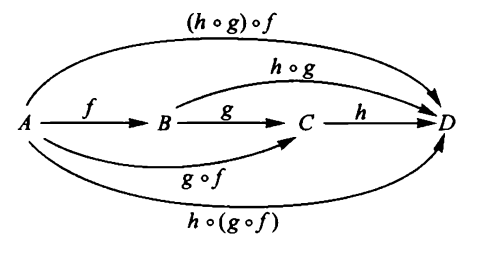
\includegraphics[scale=.4]{images/associativitydiagram} 
\end{center}
\end{figure}
Beyond associativity, another requirement is the "do nothing" map. At first seeming quite useless, it is the keystone of any group—the fundamental symmetry, if you will. This element is called the \textit{identity element} or the \textit{identity map}. The last criterion for a group is that of inverses. In a sense, this requirement that every map has an inverse map boils down to an interpretation that, in order to be a 'true' symmetry, it must be invertible. This should make sense, since, for example, if we had a map that 'forgot' some properties of an object, there wouldn't be an inverse map because this 'forgetful map' wouldn't be a bijection (one-to-one and onto). With that in mind, if one \textit{doesn't} restrict themselves to invertibility, we get another algebraic structure called a 'Monoid.' But the study of these are much more unwieldy and untame than that of groups, so this is a reasonable restriction.

\subsection{The Definition of a Group}
  A group is a set $G$, equipped with a binary operation mapping two elements to another of the form $\ast:\ G \ast G \to G$ such that the following conditions hold:\autocite[16]{saracino}
\\\textbf{Associativity}
\\$\text{For all } a,b,c \in G,\ a\ast(b \ast c) = (a\ast b) \ast c$
\\\textbf{Identity}
\\$\text{There exists an element } e \in G \text{ such that } a \ast e = e \ast a = a \ \forall a \in G$
\\\textbf{Inverse}
\\$\text{Each element } x \in G \text{ has a unique inverse } x\inv \in G \text{ such that } x \ast x\inv = x\inv \ast x = e$


In our 'symmetry-focused' definition, this set consisted of the symmetry-preserving transformations on an object where the binary operation was composing transformations. It's worth mentioning that this axiomatic definition of a group was agreed upon some 100 years after mathematicians began to study groups. It is for this reason that the 'symmetry' understanding of a group can often be more applicable to answer "why study groups at all?". Under this axiomatic definition of a group, you could probably tease out a few examples. For instance, the integers form a group under addition $(\mathbb{Z}, +)$. It's worth verifying for yourself that these do fit the definition of a group. Our identity element is 0, since $0 + a = a + 0 = a$ for all $a \in \mathbb{Z}$. Addition of integers is clearly associative. And, every number has a unique inverse, $a\inv := -a$. This group can also be thought of as the sliding symmetries of the integer lattice on the number line, in which case I like to think of an operation $3+5$ corresponding to taking the number 5 and seeing where it ends up after sliding the entire numberline ahead 3 units (or vice-versa). Similarly, the real numbers (excluding 0) form a group under multiplication. Again its worth verifying that it has an identity element $1$, that it's operation is associative, and that every element has an inverse $a\inv := \frac{1}{a}$, since $a\times \frac{1}{a} = \frac{1}{a} \times a = 1, \ \forall  a \in \reals$. To help your intuition, also consider that the positive integers $(\mathbb{Z},\times)$  \textit{do not} form a group under multiplication, since inverses are not suitably defined, i.e., there is no integer $a$ such that $a\times 2 = 2 \times a = 1$.
  The reason why the axiomatic approach is the predominant way to introduce groups is because by forgoing the need to study a group's representation, Group theory can concern itself more with the group itself and its properties in \textit{any} situation it appears. Because of this, Mathematicians concern themselves with classifying groups \textit{up to isomorphism}, meaning up to a renaming of the elements.\footnote[2]{It turns out if we restrict ourselves to finite \textit{simple} groups (somewhat like the 'prime' groups), Mathematicians have already completed the classification. This was one of the major accomplishments in 20th century mathematics, provoking many questions about paradoxical 'sporadic groups.'\\\autocite{aschbacher}}

\subsection{The Case for Commutativity and Abelian Groups}
One key property that we didn't require in our group axioms is \textit{commutativity}. At first glance, this might seem like an obvious condition, since many of the introductory examples do obey commutativity. But most of the insight that comes from group theory is from the study of groups that do not obey commutativity. This distinction happens to be so important that we give groups obeying commutativity a special name: \textit{Abelian groups}.\autocite[17]{dummit} Likewise, groups that violate this condition are sometimes called \textit{non-abelian groups}. In general, non-abelian groups correspond to symmetries that change the backdrop for another symmetry to occur. For instance, the group of symmetries on a square, $\mathrm{D}_8$, is non-abelian (meaning non-commutative). If you labeled the verticies of a square, you'd find performing a rotation and than a reflection is not, in general, the same as performing a reflection than a rotation\footnote[2]{If we were working with the presentation of $\mathrm{D}_8$, $\langle a,x\ \vert \ a^4 = x^2 = e,\ xax\inv = a\inv \rangle$, we would say that $x$ and $a$ don't commute—corresponding to the reflection and rotation generators respectively.}
—corresponding to the fact that reflections change the backdrop on which a rotation acts. Despite this, many of the other examples we've looked at so far happen to be abelian groups. For instance, the additive groups of the integers $(\mathbb{Z},+)$, rationals $(\mathbb{Q},+)$, and reals $(\reals, +)$, all obey commutativity and are hence 'Abelian.' Similarly, the circle group $\mathbb{T}$, corresponding to the rotative symmetries of a circle, is commutative as well (a fact which is of great importance to Quantum Field Theory).
  Much of the groups that are of importance to cryptography are abelian groups. For intuition on why this may be the case, consider the RSA example before. Both parties combined a series of steps involving their public and private keys. If the order in which the modular exponentiation was performed mattered, Alice and Bob would get different results after combining their public and private keys in such a way.

\section{Group Law on an Elliptic Curve}
While the elliptic curve group admits an intuitive geometric description, it's important that our algebraic description satisfies the group axioms.  $ E(\field_{q} )$ 

jacobbruner.com/elliptic-curve

[I have yet to finish this chapter.]

\autocite[10]{koblitz}

\newpage 

\printbibliography

\end{document}